\documentclass[14pt]{extarticle}

\usepackage{arxiv}

\usepackage[utf8]{inputenc}        % allow utf-8 input
\usepackage[T1,T2A]{fontenc}       % Latin (T1) + Cyrillic (T2A)
\usepackage{mathptmx}              % Times New Roman-like serif (GOST font)
\usepackage[english,russian]{babel}
\usepackage{setspace}\onehalfspacing  % line spacing 1.5 (within 1.3-1.5)
\usepackage{hyperref}
\usepackage{url}
\usepackage{booktabs}
\usepackage{amsfonts}
\usepackage{amsmath}
\usepackage{amsthm}
\theoremstyle{plain}
\newtheorem{lemma}{Лемма}
\newtheorem{proposition}{Предложение}
\newtheorem{corollary}{Следствие}
\renewcommand{\proofname}{Доказательство}
\usepackage{nicefrac}
\usepackage{microtype}
\usepackage{graphicx}
\usepackage[table]{xcolor}
\usepackage{doi}
\usepackage[sort&compress]{natbib}
\setcitestyle{numbers}
\bibliographystyle{unsrtnat}            % TODO: GOST R 7.0.5-2008 via biblatex-gost

% --- GOST formatting: red-line indent, object numbering within chapter ---
\setlength{\parindent}{1cm}
\numberwithin{equation}{section}
\numberwithin{figure}{section}
\numberwithin{table}{section}

\title{Исследование влияния параметров методов оценки ошибок генерации диффузионных моделей}

\author{
    Пахуров Фёдор Константинович\\
    МФТАД251,\\
    НИУ ВШЭ,\\
    Москва, Россия\\
    \texttt{fpakhurov@gmail.com}
}

\date{}

\renewcommand{\headeright}{Курсовой проект}
\renewcommand{\undertitle}{Курсовой проект (исследовательский проект)}
\renewcommand{\shorttitle}{Параметры CE-оценки ошибок диффузии}

\hypersetup{
pdftitle={Исследование влияния параметров методов оценки ошибок генерации диффузионных моделей},
pdfauthor={Fedor K. Pakhurov},
pdfkeywords={диффузионные модели, оценка галлюцинаций, оценка ошибок генерации, сложность-энтропия, перестановочная энтропия},
}

\begin{document}
\begin{titlepage}

\begin{center}
НАЦИОНАЛЬНЫЙ ИССЛЕДОВАТЕЛЬСКИЙ УНИВЕРСИТЕТ\\
«ВЫСШАЯ ШКОЛА ЭКОНОМИКИ»
\\
\bigskip
Факультет компьютерных наук\\
Магистерская программа «Финансовые технологии и анализ данных»
% TODO: подтвердить точное название программы МФТАД, если требуется иное.
\end{center}


\vspace{7em}

\begin{center}
{\bf КУРСОВАЯ РАБОТА}\\
{\bf (исследовательский проект)}\\
\medskip
{\bf на тему:}\\
{\bf Исследование влияния параметров методов оценки\\
ошибок генерации диффузионных моделей}\\
\end{center}

\vspace{2em}

{\bf Выполнил студент: \vspace{2mm}}

\begin{tabular}{l@{\hskip 1.5cm}l}
группа \#МФТАД251, 1-й курс магистратуры &
Пахуров Фёдор Константинович
\end{tabular}

\vspace{1em}
{\bf Принял научный руководитель: \vspace{2mm}}

\begin{tabular}{l@{\hskip 1.5cm}l}
Лукьянченко Пётр Павлович, \\
старший преподаватель, \\
Школа больших данных и информационного поиска \\
\end{tabular}

\mbox{}
  \\ \\ \\ \\ \\ \\ \\ \\ \\ \\ \\ \\ \\ \\ \\ \\ \\ \\ \\ \\ \\ \\ \\ \\ \\ \\ \\ \\ \\
\mbox{}

\begin{center}
Москва 2026
\end{center}

\end{titlepage}

\maketitle

\renewcommand{\abstractname}{Аннотация}
\begin{abstract}
Диффузионные модели порождают ошибки разной природы: синтетичность,
низкоуровневые текстурные артефакты, структурное дублирование и семантические
несоответствия. В работе систематически изучается влияние параметров лёгкого
детерминированного дескриптора на основе кривых сложности–энтропии Реньи (CE) на
оценку этих ошибок. Эвристическая метрика заменена воспроизводимым протоколом
(логистическая регрессия, повторная кросс-валидация, бутстреп-интервалы, тест
ДеЛонга, контроль доли ложных открытий). Раздельно проверены две гипотезы:
различение реального и синтетического (H1) и различение удачных и неудачных
генераций (H2). Гипотеза H1 подтверждается на выборках (AUROC до $0{,}86$) и на
CIFAKE ($0{,}76$); контроль источника при этом выявляет значимый конфаунд данных,
а CE не превосходит спектр Фурье. Гипотеза H2 не подтверждается: ни одна из $44$
конфигураций не превышает случайность. На основе нелокальных ординальных признаков
построен лёгкий детектор дублирования, устойчивый к тоновой правке вставки.

\medskip\noindent\textbf{Ключевые слова:} сложность–энтропия, перестановочная
энтропия, оценка ошибок генерации, диффузионные модели, детектор дублирования.
\end{abstract}

\renewcommand{\abstractname}{Abstract}
\begin{abstract}
Diffusion models produce errors of different natures: syntheticity, low-level
texture artifacts, structural duplication, and semantic inconsistencies. This
work systematically studies how the parameters of a lightweight deterministic
descriptor based on Rényi complexity–entropy (CE) curves affect the evaluation
of such errors. The original heuristic metric is replaced by a reproducible
protocol (logistic regression, repeated cross-validation, bootstrap intervals,
DeLong test, false-discovery-rate control). Two hypotheses are tested
separately: distinguishing real from synthetic images (H1) and distinguishing
successful from failed generations (H2). H1 holds on the collected samples
(AUROC up to $0.86$) and on CIFAKE ($0.76$); however, a source-confound control
reveals a substantial data confound, and CE does not outperform a Fourier
spectrum. H2 is not supported: none of $44$ configurations exceeds chance.
Building on non-local ordinal features, a lightweight duplication detector is
proposed that is robust to tone editing of the pasted region.

\medskip\noindent\textbf{Keywords:} complexity–entropy, permutation entropy,
generation-error evaluation, diffusion models, duplication detector.
\end{abstract}

\clearpage
\tableofcontents

% ==================================================================
\clearpage
\section{Введение}\label{sec:intro}

\paragraph{Актуальность и значимость.} Диффузионные модели лежат в основе
творческого дизайна, научной визуализации и систем поддержки принятия решений,
однако регулярно порождают ошибки генерации. Существующие протоколы оценки
измеряют расхождение распределений с обучающими данными и слабо помогают
количественно оценивать ошибки в конкретных новых генерациях. Для лёгких
статистических дескрипторов особенно важна честная оценка: дешёвый метод легко
выдать за работающий, измеряя его неподходящей метрикой на малой выборке. Работа
показывает, как воспроизводимый протокол и параметрический анализ отделяют
реальный сигнал от иллюзии, внося вклад в методологию оценки порождающих моделей.

\paragraph{Объект и предмет.} Объект исследования — методы оценки ошибок генерации
диффузионных моделей на основе ординальных дескрипторов сложности–энтропии (CE).
Предмет — влияние параметров таких методов (размерность вложения $d$, задержка
$\tau$, набор параметров Реньи, схема линеаризации $2$D$\to1$D, двумерные шаблоны)
на качество и статистическую значимость оценки.

\paragraph{Таксономия ошибок.} Под «ошибкой генерации» объединяют разные явления,
для CE существенно различные: (i) \emph{синтетичность} — статистическое отличие
сгенерированного изображения от реального; (ii) \emph{низкоуровневый артефакт} —
локальное искажение текстуры; (iii) \emph{структурное дублирование} — повтор
фрагмента; (iv) \emph{семантическая ошибка} — нарушение смысла и несоответствие
промпту. CE оперирует порядковой статистикой, поэтому сигнал естественно ожидать
для (i)–(ii) и его отсутствие для (iv). Работа изучает \emph{оценку} ошибок
генерации и не претендует на \emph{обнаружение} семантических галлюцинаций.

\paragraph{Цель.} Установить, как параметры CE-методов влияют на оценку ошибок
генерации, и определить, какие ошибки такие методы способны различать
статистически значимо.

\noindent\textbf{Задачи.}
\begin{enumerate}
\item проанализировать современные методы оценки ошибок диффузионной генерации,
      выявив их допущения и ограничения;
\item заменить эвристическую метрику воспроизводимым протоколом (AUROC/AP,
      доверительные интервалы, тест значимости) и сформулировать проверяемые
      гипотезы;
\item систематически измерить влияние параметров метода на качество оценки;
\item проверить устойчивость выводов на независимом размеченном датасете и
      контролировать конфаунд источника данных.
\end{enumerate}

\paragraph{Методы исследования.} Ординальный (порядковый) анализ и кривые
сложности–энтропии Реньи; статистическое обучение (логистическая регрессия);
повторная стратифицированная кросс-валидация, бутстреп-доверительные интервалы,
тест ДеЛонга и контроль доли ложных открытий; контролируемая инъекция артефактов
с известной основной истиной.

\paragraph{Основной результат.} CE — дешёвый интерпретируемый дескриптор
\emph{синтетичности}, качество которого управляется прежде всего задержкой и
схемой линеаризации и не превосходит спектр Фурье; глобальная CE-статистика не
даёт значимого сигнала для различения удачных и неудачных генераций, что
объясняется её инвариантностью к структуросохраняющим искажениям. На основе
нелокальных ординальных признаков построен лёгкий детектор дублирования,
устойчивый к тоновой правке вставки.

\paragraph{Структура работы.} Раздел~\ref{sec:related} — обзор подходов;
раздел~\ref{sec:method_choice} — выбор и исправление метода;
раздел~\ref{sec:method} — методология и протокол; раздел~\ref{sec:theory} —
математические свойства; раздел~\ref{sec:results} — эксперименты;
раздел~\ref{sec:copymove} — прикладной детектор дублирования;
разделы~\ref{sec:discussion}--\ref{sec:future} — обсуждение, расширения и
ограничения; раздел~\ref{sec:conclusions} — заключение.

% ==================================================================
\section{Обзор существующих подходов}\label{sec:related}

\subsection{Анализ интерполяции мод в латентном пространстве}
Метод mode-interpolation отслеживает дисперсию траекторий обратной диффузии для
выявления генераций вне носителя распределения \citep{NEURIPS2024_f29369d1}.
Дисперсия по последним $K$ шагам:
\begin{equation}
\sigma^{2}= \frac{1}{K}\sum_{k=1}^{K}\bigl\lVert
x_{t_k}-\bar{x}\bigr\rVert_2^{2}, \qquad
\bar{x}=\frac{1}{K}\sum_{k=1}^{K}x_{t_k}.
\label{eq:traj_var}
\end{equation}
Ограничения: пороги зависят от модели, метрика глобальна, хранение всей
траектории затратно.

\subsection{Оценка через граф сцены и вопросно-ответную модель}
Qin \emph{и др.} преобразуют изображение в граф сцены и опрашивают языковую
модель; рассогласование ответов и запроса указывает на галлюцинацию
\citep{qin2024evaluatinghallucinationtexttoimagediffusion}. Качество ограничено
точностью распознавания и извлечения отношений, а время работы определяется
инференсом LLM.

\subsection{Локальная диффузионная декомпозиция}
Kim \emph{и др.} снижают структурные галлюцинации с помощью локальной диффузии,
учитывающей области вне распределения \citep{10.1007/978-3-031-73004-7_6}.
Однако качество OOD-масок и многократная выборка ограничивают практичность.

\subsection{Анализ сложности–энтропии}\label{sec:ce}

\paragraph{Перестановочная энтропия.}
Для скалярного ряда $X=(x_1,\dots,x_N)$, размерности вложения $d$, задержки
$\tau$ и частот перестановок $P=\{p_i\}$ \citep{bandt2002permutation}:
\begin{equation}
H_S(d,\tau)=-\sum_{i=1}^{d!}p_i\log p_i, \quad
h_S=\frac{H_S}{\log d!}\in[0,1].
\label{eq:perm_entropy}
\end{equation}

\paragraph{Сложность Йенсена–Шеннона.}
При равномерном распределении $P_u$ и $m_i=\tfrac12(p_i+1/d!)$:
\begin{align}
D_{\mathrm{JS}}(P,P_u) &=
\tfrac12\sum_{i}\Bigl[p_i\log\frac{p_i}{m_i}+
\frac{1}{d!}\log\frac{1/d!}{m_i}\Bigr],\\[2pt]
C_{\mathrm{JS}} &=
\frac{D_{\mathrm{JS}}(P,P_u)}{D_{\mathrm{JS}}^{\max}}\;h_S.
\end{align}
Точки $(h_S,C_{\mathrm{JS}})$ образуют причинную плоскость сложности–энтропии
\citep{PhysRevE.95.062106}.

\paragraph{Кривая сложности–энтропии Реньи.}
Замена энтропии Шеннона энтропией Реньи даёт семейство кривых, различающих
хаотические, стохастические и периодические сигналы
\citep{RePEc:eee:phsmap:v:498:y:2018:i:c:p:74-85}. Сложности этого подхода —
чувствительность к $(d,\tau)$, факториальный рост $d!$ и инфляция энтропии шумом
\citep{2016NTA.....7...21C}.

\paragraph{Двумерный и мультимасштабный ординальный анализ изображений.}
Перенос ординального анализа на изображения формализован: причинная плоскость
сложности–энтропии обобщена на двумерные паттерны $D_x\times D_y$
\citep{ribeiro2012complexity}, а её \emph{мультимасштабная} версия использует
пространственные задержки $\tau_x,\tau_y$ (кратные шагу дискретизации) для
сканирования текстур на разных масштабах и успешно различает текстуры Бродаца,
фракталы и снимки Марса \citep{zunino2016discriminating}. Эти работы — прямое
математическое основание нашего метода; наш базовый конвейер соответствует
\emph{одномасштабному} случаю ($\tau=1$), а мультимасштабное обобщение мы относим
к расширениям (раздел~\ref{sec:extensions}).

\paragraph{Амплитудно-зависимые варианты ординальной энтропии.}
Классическая перестановочная энтропия Бандта–Помпе \emph{отбрасывает} амплитуду,
учитывая лишь порядок. Ряд детерминированных, лёгких обобщений возвращает
амплитудную информацию: взвешенная перестановочная энтропия
\citep{fadlallah2013weighted}, амплитудно-зависимая перестановочная энтропия
\citep{azami2016amplitude} и дисперсионная энтропия на основе НФР
\citep{rostaghi2016dispersion}. Все они сохраняют ключевые преимущества
(детерминизм, линейная сложность) и являются естественными кандидатами на
усиление CE-признаков.

\paragraph{Детекторы синтетических изображений.}
Параллельная линия работ показывает, что диффузионные генерации оставляют
устойчивые частотные «отпечатки» \citep{corvi2023detection,bird2024cifake}.
Существенно, что у диффузионных изображений высокочастотные компоненты
\emph{ниже}, чем у реальных (тогда как у GAN — выше), а операции повышающей
дискретизации порождают \emph{осевые локальные корреляции} пикселей. Это
напрямую объясняет наш результат (раздел~\ref{sec:sweep}): построчный растр,
идущий вдоль осей, улавливает синтетичность лучше локально-связной кривой
Гильберта. Энтропийный признак также используется напрямую: метод MLEP строит
карты локальной энтропии по перемешанным мультимасштабным патчам как
\emph{источниконезависимый} признак, обобщающийся на $32$ генератора
\citep{yuan2025mlep}, а самоподобие спектра предлагается как обобщаемый признак
синтетичности \citep{tan2025fractal}. Общий вывод контекста: сигнал «реальное
против синтетического» физически объясним, тогда как семантические галлюцинации
такого простого статистического следа могут не оставлять.

\subsection{Сравнительные ограничения и выводы}
Ни один из методов не покрывает все типы галлюцинаций. Методы mode-interpolation
и локальной диффузии требуют доступа к процессу выборки; SG-QA требует разметки
запросов и дорог по времени. CE-подход уникален дешевизной и
архитектурной независимостью, но именно поэтому требует особенно аккуратной
проверки на статистическую значимость — чему и посвящена настоящая работа.

% ==================================================================
\section{Выбор и обоснование метода}\label{sec:method_choice}

\subsection{Пространство признаков сложности–энтропии}
\begin{enumerate}
\item \textbf{Архитектурная независимость.} CE-дескрипторы оперируют порядковой
      статистикой отсчётов и не зависят от внутренних состояний модели.
\item \textbf{Чувствительность к нерегулярной структуре.} Комбинация
      нормированной перестановочной энтропии и статистической сложности
      разделяет стохастические, периодические и хаотические режимы.
\item \textbf{Вычислительная эффективность.} Требуется лишь подсчёт порядковых
      шаблонов; сложность линейна по длине сигнала.
\item \textbf{Интерпретируемость.} Двумерная плоскость CE даёт наглядную
      поверхность решения.
\end{enumerate}

\subsection{Критика и исправление исходного конвейера}\label{sec:fix}
Исходная реализация преобразовывала изображение в одномерный сигнал, пропуская
его через единственный свёрточный слой \texttt{nn.Conv2d}. Анализ кода выявил
существенный дефект: \textbf{свёртка была инициализирована случайно и не
обучалась, причём новые случайные веса создавались при каждом вызове без фиксации
зерна}. В результате «сетка перебора» сравнивала один случайный проекционный шум
с другим. Это объясняет, почему наблюдавшиеся в исходной работе «оценки
разделения» имели порядок $0{,}004$ против $-0{,}001$ — то есть лежали в пределах
статистического шума. В настоящей работе случайная свёртка \emph{полностью
удалена}: признаки вычисляются непосредственно из изображения (через явную схему
линеаризации либо нативные двумерные порядковые шаблоны), а весь конвейер
детерминирован.

% ==================================================================
\subsection*{Выводы по главе}
Обзор показывает, что лёгкие ординальные дескрипторы дёшевы и архитектурно
независимы, однако их применимость требует строгой проверки. Исходный конвейер
содержал необучаемую случайную свёртку, дававшую шумовые результаты; она удалена,
а оценка переведена на воспроизводимый протокол.

\section{Методология и протокол оценки}\label{sec:method}

\subsection{Признаки кривых сложности–энтропии}
Для набора параметров Реньи $\alpha\in\mathcal{A}=\{0{,}0;0{,}1;\dots;1{,}0\}$
($|\mathcal{A}|=10$) каждому сигналу сопоставляется вектор
\begin{equation}
\mathbf{f}(X)=[H_\alpha,\,C_\alpha]_{\alpha\in\mathcal{A}}\in\mathbb{R}^{2|\mathcal{A}|},
\end{equation}
где $H_\alpha$ — нормированная энтропия Реньи порядковых шаблонов, $C_\alpha$ —
соответствующая статистическая сложность. Вычисления выполнены пакетом
\texttt{ordpy} \citep{pessa2021ordpy}.

\subsection{Схемы линеаризации изображения}
Изображение переводится в оттенки серого и масштабируется. Мы сравниваем пять
схем обхода: построчный (\texttt{row}), постолбцовый (\texttt{col}),
«змейкой» (\texttt{snake}), по антидиагоналям (\texttt{diag}) и вдоль
кривой Гильберта (\texttt{hilbert}). Дополнительно используется \emph{нативный
двумерный} режим: порядковые шаблоны размера $d_x\times d_y$ строятся прямо по
двумерной матрице яркостей, без линеаризации.

\subsection{Протокол оценки и гипотезы}
Поверх CE-признаков обучается логистическая регрессия со стандартизацией
признаков (\texttt{scikit-learn} \citep{pedregosa2011scikit}). Качество
оценивается \emph{повторной стратифицированной $5$-кратной кросс-валидацией}
($5$ повторов). Out-of-fold предсказание каждого объекта \emph{усредняется по
повторам} (одно значение на реальный объект), после чего для AUROC и средней
точности (AP) строятся $95\%$ бутстреп-доверительные интервалы ($2000$ ресэмплов)
ресэмплингом реальных объектов. Усреднение по объекту здесь принципиально: наивное
объединение всех повторов засчитывало бы каждый объект пятикратно и искусственно
сужало доверительные интервалы. Этот протокол заменяет
эвристическую метрику исходной работы (разделение средних вероятностей кластеров).

Мы раздельно проверяем две гипотезы:
\begin{itemize}
\item[\textbf{H1.}] CE-признаки отличают \emph{реальные} изображения от
      \emph{синтетических} (real vs synthetic).
\item[\textbf{H2.}] CE-признаки отличают \emph{неудачные} (галлюцинирующие)
      генерации от \emph{удачных} (bad vs good).
\end{itemize}
Гипотеза считается подтверждённой, только если нижняя граница доверительного
интервала AUROC строго превосходит $0{,}5$.

% ==================================================================
\section{Математические свойства метода}\label{sec:theory}

Три свойства ординальных дескрипторов формализуют и объясняют наблюдения
разделов~\ref{sec:results}. Везде $X=(x_1,\dots,x_N)$ — вещественный сигнал,
а ординальный шаблон окна — перестановка, сортирующая его элементы; через $P$
обозначена вероятностная мера ординальных шаблонов.

\begin{lemma}[Инвариантность к монотонным преобразованиям]\label{lem:mono}
Пусть $g:\mathbb{R}\to\mathbb{R}$ строго возрастает. Тогда ординальный шаблон
любого окна не меняется при поэлементном применении $g$, а потому распределение
$P$, перестановочная энтропия и кривая сложности–энтропии инвариантны к замене
$x_t\mapsto g(x_t)$.
\end{lemma}
\begin{proof}
Строго возрастающая $g$ сохраняет порядок: $x_i<x_j\iff g(x_i)<g(x_j)$. Шаблон
определён лишь относительным порядком значений, поэтому он совпадает для $X$ и
$g(X)$. Все величины, зависящие только от $P$, сохраняются. \qedhere
\end{proof}

\begin{corollary}\label{cor:mono}
CE-признаки инвариантны к яркости, контрасту, гамме и любой монотонной тоновой
кривой. Спектральные и текстурно-гистограммные признаки этим свойством не
обладают, что даёт CE устойчивость к различиям конвейеров обработки; этот эффект
частично объясняет поведение при переносе (раздел~\ref{sec:transfer}).
\end{corollary}

\begin{proposition}[Инвариантность к перестановке и слепота к дублированию]\label{prop:dup}
Мера $P$ зависит лишь от мультимножества шаблонов окон и не зависит от их
пространственного расположения. Пусть патч $B$ (с распределением шаблонов внутренних
окон $P_B$) копируется на целевую область $T$ из $m_T$ окон, исходное распределение
которой $P_T$. Тогда изменение меры в полной вариации ограничено
\begin{equation}
\bigl\lVert P'-P\bigr\rVert_{\mathrm{TV}}
\;\le\; \frac{m_T}{M}\,\bigl\lVert P_B-P_T\bigr\rVert_{\mathrm{TV}}
\;+\; O\!\left(\frac{|\partial|}{M}\right),
\label{eq:dupbound}
\end{equation}
где $M$ — общее число окон, $|\partial|$ — число окон, пересекающих новую границу.
Следовательно, любая величина, зависящая только от $P$ (перестановочная энтропия,
кривая Реньи, гистограмма переходов шаблонов), не может обнаружить дублирование,
если копируемый и заменяемый фрагменты статистически близки
($P_B\approx P_T$): тогда оба слагаемых в \eqref{eq:dupbound} малы.
\end{proposition}
\begin{proof}
$P=\frac{1}{M}\sum_i \delta_{\pi_i}$ симметрична по индексу окна $i$. Копирование
удаляет $m_T$ внутренних окон области $T$ (вклад $\tfrac{m_T}{M}P_T$) и добавляет
$m_T$ внутренних окон патча $B$ (вклад $\tfrac{m_T}{M}P_B$); разность этих вкладов
даёт первый член. Дополнительно изменяются лишь $O(|\partial|)$ окон, пересекающих
границу, что даёт второй член. \qedhere
\end{proof}

\begin{corollary}
Предложение~\ref{prop:dup} объясняет результат эксперимент 5: на структуросохраняющем
артефакте \texttt{repeat}, где копируемый фрагмент берётся из того же изображения и
потому статистически близок ($P_B\approx P_T$), гистограмма CE и сеть переходов Б1
остаются у случайности (раздел~\ref{sec:inject},~\ref{sec:novel_eval}). Дескриптор
Б2 по построению использует пространственное расположение (сопоставление блоков по
смещениям) и выходит за рамки этого ограничения.
\end{corollary}

\begin{proposition}[Спектральная связь]\label{prop:spec}
Пусть $X$ — стационарная гауссовская последовательность с нулевым средним и
автоковариацией $\gamma(k)$. Для размерности вложения $d=3$ и задержки $\tau$
введём приращения $\Delta_1=x_{t+\tau}-x_t$, $\Delta_2=x_{t+2\tau}-x_{t+\tau}$.
Пара $(\Delta_1,\Delta_2)$ гауссовская с корреляцией
\begin{equation}
r_\tau=\frac{2\gamma(\tau)-\gamma(0)-\gamma(2\tau)}{2\bigl(\gamma(0)-\gamma(\tau)\bigr)} .
\label{eq:rtau}
\end{equation}
Вероятность монотонного ординального шаблона (совпадение знаков $\Delta_1,\Delta_2$)
по формуле Шеппарда равна $\tfrac12+\tfrac1\pi\arcsin r_\tau$. Тем самым
распределение шаблонов, перестановочная энтропия и кривая CE суть явные функции
автоковариации на лагах $\tau$ и $2\tau$; по теореме Винера–Хинчина
$\gamma(k)=\int_{-\pi}^{\pi}S(\omega)\cos(k\omega)\,d\omega$ они определяются
спектром мощности $S$ \citep{bandt2007order}.
\end{proposition}
\begin{proof}
$\operatorname{Var}\Delta_1=\operatorname{Var}\Delta_2=2(\gamma(0)-\gamma(\tau))$,
а $\operatorname{Cov}(\Delta_1,\Delta_2)=2\gamma(\tau)-\gamma(0)-\gamma(2\tau)$,
откуда \eqref{eq:rtau}. Для двумерной гауссовской пары с нулевым средним и
корреляцией $r$ вероятность совпадения знаков равна
$\tfrac12+\tfrac1\pi\arcsin r$ (формула Шеппарда). \qedhere
\end{proof}

\begin{corollary}
Задержка $\tau$ задаёт спектральные масштабы, на которых работает дескриптор. Для
построчной развёртки изображения ширины $W$ лаг $\tau=W$ отвечает ковариации
вертикальных соседей, что объясняет наблюдаемый резонанс качества на $\tau=256=W$
(раздел~\ref{sec:extended}).
\end{corollary}

% ==================================================================
\subsection*{Выводы по главе}
Сформулированы две раздельные гипотезы и строгий протокол их проверки. Доказаны
три свойства CE: инвариантность к монотонным преобразованиям, инвариантность к
перестановке (с поправкой на различие распределений патчей) и связь со спектром
через автоковариацию, объясняющая резонанс по задержке.

\section{Эксперименты и результаты}\label{sec:results}

\subsection{Данные}
Сбалансированный корпус из $100$ изображений в трёх взаимоисключающих классах:
\emph{Real} (реальные фотографии, $33$), \emph{Good} (удачные диффузионные
генерации, $32$) и \emph{Bad} (галлюцинирующие/неудачные генерации, $35$). Класс
\emph{Real} взят из MS~COCO \citep{Lin2014COCO} и FFHQ \citep{Karras2019FFHQ};
\emph{Good} — из подборок Midjourney \citep{MidjourneyWebsite}, галереи
DALL\textperiodcentered E~3 \citep{DALLE3Gallery}, SDXL \citep{Podell2023SDXL},
Imagen \citep{Saharia2022Imagen}, Mage \citep{MageSpace} и Lexica
\citep{LexicaArt}; \emph{Bad} — из таксономии артефактов Everypixel
\citep{EverypixelHalluc}, тематической ветки r/StableDiffusion
\citep{RedditStableFail} и подборки Bored Panda \citep{BoredPandaFails}.
Задача H1 — \emph{Real} против \emph{Good}$\cup$\emph{Bad}; задача H2 —
\emph{Bad} против \emph{Good}.

\subsection{Эксперимент 1. Наличие сигнала}\label{sec:e1}
Таблица~\ref{tab:e1} приводит качество базовой конфигурации (\texttt{row},
$d=5$, $\tau=1$) и нативных 2D-шаблонов. Сигнал для H1 силён и значим
(AUROC $0{,}857$, ДИ строго выше $0{,}5$); сигнал для H2 неотличим от
случайного.

\begin{table}[h!]
\centering
\begin{tabular}{@{}llccc@{}}
\toprule
Задача & Конфигурация & $n$ & AUROC [95\% ДИ] & AP [95\% ДИ] \\
\midrule
H1 (real vs synthetic) & \texttt{row}, $d{=}5$, $\tau{=}1$ & 100 & \textbf{0.858} [0.779, 0.927] & 0.653 [0.507, 0.850] \\
H1 (real vs synthetic) & 2D, $d_x{=}d_y{=}2$               & 100 & 0.767 [0.668, 0.854] & 0.580 [0.438, 0.756] \\
H2 (bad vs good)       & \texttt{row}, $d{=}5$, $\tau{=}1$ & 67  & 0.446 [0.315, 0.591] & 0.499 [0.376, 0.676] \\
H2 (bad vs good)       & 2D, $d_x{=}d_y{=}2$               & 67  & 0.393 [0.258, 0.539] & 0.445 [0.339, 0.608] \\
\bottomrule
\end{tabular}
\caption{Базовая оценка по двум задачам. H1 значимо превышает случайность,
H2 — нет (доверительный интервал накрывает $0{,}5$).}
\label{tab:e1}
\end{table}

\begin{figure}[h!]
\centering
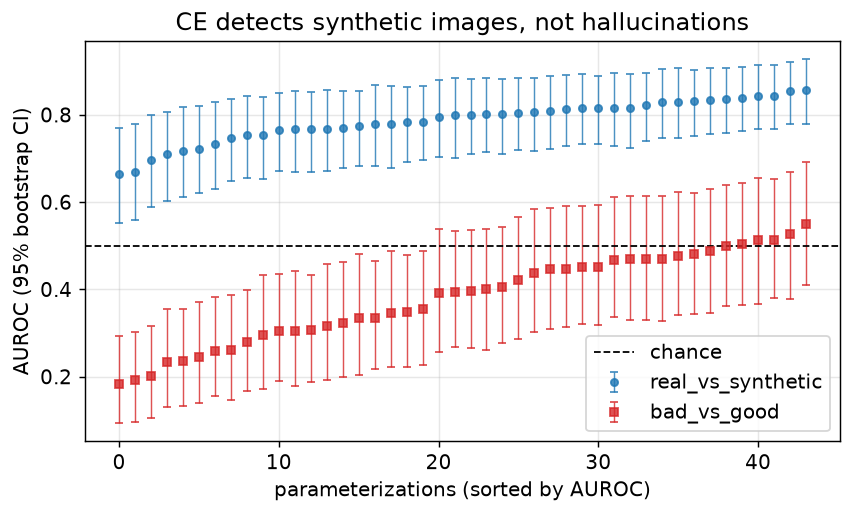
\includegraphics[width=.85\linewidth]{fig_two_tasks.png}
\caption{AUROC всех $44$ параметризаций, отсортированных по возрастанию, с $95\%$
бутстреп-доверительными интервалами. Облако H1 (real vs synthetic) лежит выше
линии случайности при всех настройках; облако H2 (bad vs good) прижато к $0{,}5$.
CE-дескрипторы различают синтетичность; для галлюцинаций сигнала нет.}
\label{fig:two_tasks}
\end{figure}

\subsection{Эксперименты 2–3. Влияние параметров}\label{sec:sweep}
Перебор охватывает пять схем линеаризации $\times$ четыре значения $d\in\{3,4,5,6\}$
$\times$ две задержки $\tau\in\{1,2\}$, а также четыре конфигурации нативных
2D-шаблонов — всего $44$ параметризации, каждая оценивалась по обеим задачам.
Для задачи H1 качество существенно зависит от параметров (AUROC от $0{,}664$ до
$0{,}858$), и зависимость интерпретируема:
\begin{itemize}
\item \textbf{Задержка $\tau$.} $\tau=1$ устойчиво превосходит $\tau=2$ во всех
      схемах (в среднем $0{,}810$ против $0{,}761$); увеличение задержки разрушает
      локальные осевые корреляции, по которым и опознаётся синтетичность.
\item \textbf{Схема линеаризации.} Горизонтальный растр (\texttt{snake} $0{,}844$,
      \texttt{row} $0{,}842$) превосходит \texttt{col} ($0{,}799$),
      \texttt{hilbert} ($0{,}798$) и \texttt{diag} ($0{,}770$). Контринтуитивно
      простой строчный обход обходит локально-связную кривую Гильберта: вероятно,
      артефакты повышающей дискретизации генераторов выровнены по осям.
\item \textbf{Размерность $d$.} Влияет слабее; лучшие значения $d\in\{4,5,6\}$ при
      $\tau=1$.
\item \textbf{Нативные 2D-шаблоны.} Конкурентоспособны ($0{,}767$--$0{,}815$), но
      не превосходят лучший одномерный растр.
\end{itemize}
Для задачи H2 \textbf{ни одна} конфигурация не даёт значимого сигнала: лучший
AUROC лишь $0{,}549$ с доверительным интервалом $[0{,}411;\,0{,}691]$, и у
\emph{всех $44$} конфигураций нижняя граница ДИ строго ниже $0{,}5$; разброс
$0{,}182$--$0{,}549$ согласуется со случайным угадыванием. Это и есть
статистически обоснованный отказ от гипотезы H2.

\begin{figure}[h!]
\centering
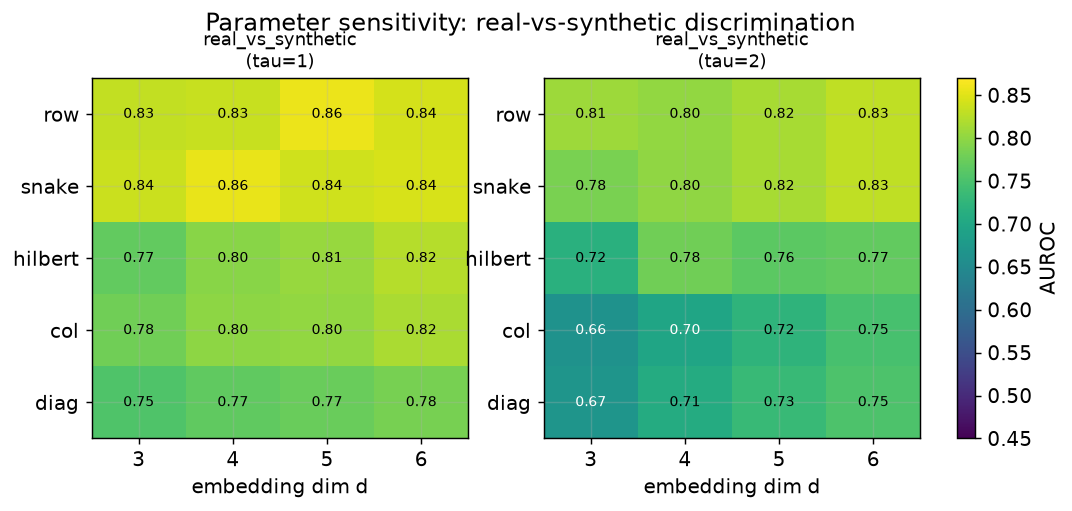
\includegraphics[width=\linewidth]{fig_heatmap.png}
\caption{Тепловые карты AUROC для задачи H1 (real vs synthetic) по схеме обхода
($y$) и размерности $d$ ($x$) при $\tau=1$ (слева) и $\tau=2$ (справа). Видны
доминирование $\tau=1$ и преимущество горизонтального растра.}
\label{fig:heatmap}
\end{figure}

\begin{figure}[h!]
\centering
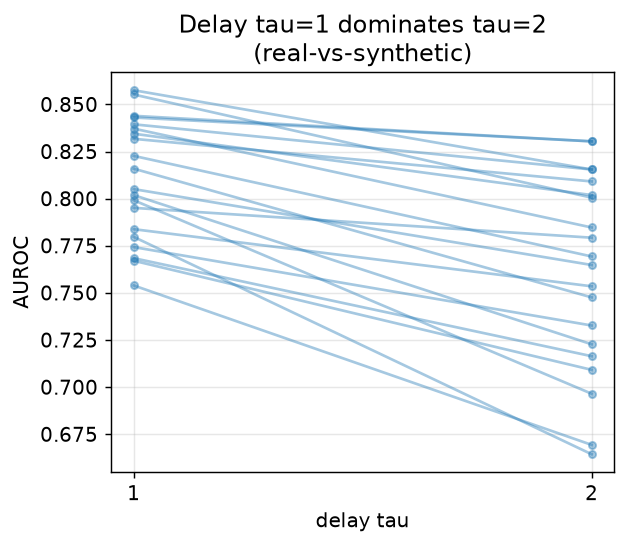
\includegraphics[width=.55\linewidth]{fig_tau_effect.png}
\caption{Парный эффект задержки $\tau$ для H1: каждая линия — одна пара
(схема, $d$). Переход $\tau{=}1\to\tau{=}2$ почти всегда снижает AUROC.}
\label{fig:tau}
\end{figure}

\subsection{Расширенное изучение $d$ и $\tau$}\label{sec:extended}
Базовый перебор ограничивал $d\le 6$ и $\tau\le 2$. Здесь мы расширяем диапазоны
на порядки: $d$ до $60$ и $\tau$ до $1024$ (рис.~\ref{fig:extended}). Это вскрывает
два математических эффекта.

\paragraph{Потолок размерности вложения.}
Размерность $d$ порождает $d!$ ординальных шаблонов. Пакет \texttt{ordpy} считает
любое $d$ быстро, поскольку хранит лишь наблюдённые шаблоны; однако при росте $d$
отношение числа окон к числу шаблонов $N/d!$ стремится к нулю, каждое окно
получает уникальный шаблон, нормированная энтропия вырождается ($0{,}88\to0{,}06$),
и различающая способность пропадает. Качество H1 держит плато до $d\approx10$
($\mathrm{AUROC}\approx0{,}85$), затем падает к случайности: $d{=}20\to0{,}69$,
$d{=}30\to0{,}54$, $d{=}50\to0{,}47$. При $d\ge171$ величина $d!$ переполняет
формат с плавающей точкой. Практический вывод: «брать $d$ в сотни» бессмысленно
по самой математике метода; рабочий диапазон $d\in[4,8]$.

\paragraph{Резонанс задержки.}
По задержке качество H1 сперва спадает ($\tau{=}1\to0{,}858$, $\tau{=}16\to0{,}54$,
$\tau{=}32\to0{,}41$), затем восстанавливается со вторичным пиком на $\tau{=}256$
($0{,}81$). Объяснение прямое: изображение линеаризовано построчно с шириной $256$,
поэтому задержка $\tau$ в ширину строки сэмплирует \emph{вертикальных} соседей
пикселя. Резонанс на $\tau=256$ есть проявление структуры растра, и он связывает
параметр $\tau$ с пространственной геометрией изображения.

\begin{figure}[h!]
\centering
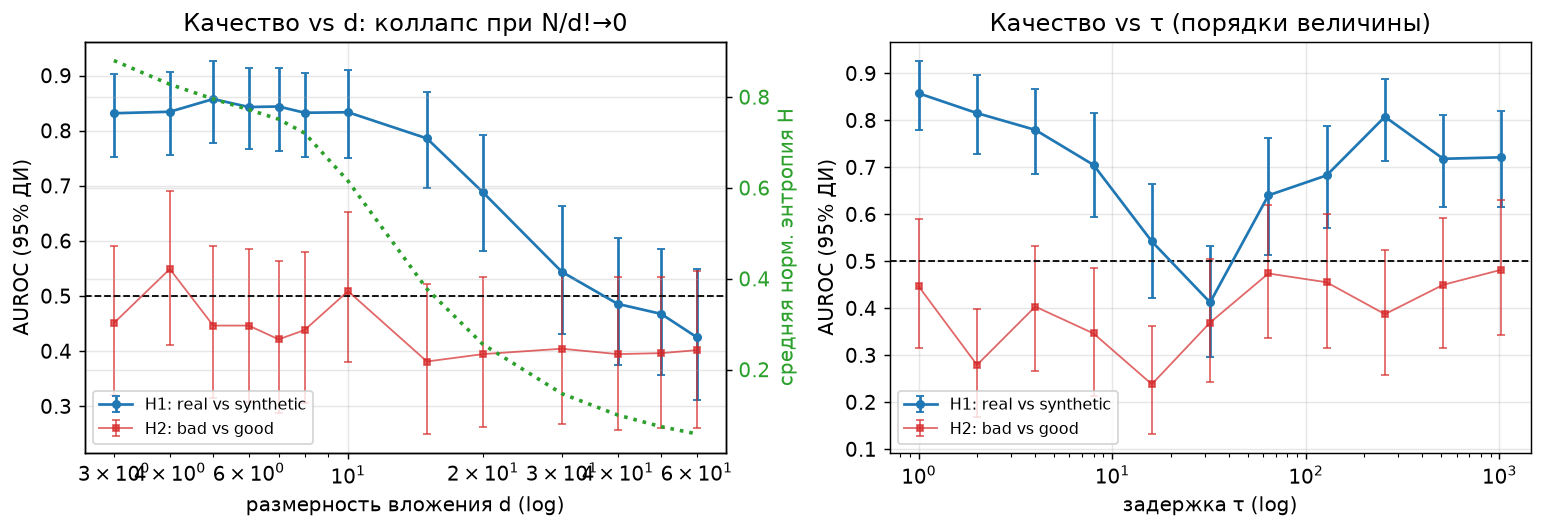
\includegraphics[width=\linewidth]{fig_extended.png}
\caption{Качество как функция размерности вложения $d$ (слева; пунктир — средняя
нормированная энтропия) и задержки $\tau$ (справа), логарифмическая ось. Слева
виден коллапс при $N/d!\to0$; справа — провал на $\tau\approx32$ и резонансный пик
на $\tau=256$ (ширина изображения, сэмплирование вертикальных соседей).}
\label{fig:extended}
\end{figure}

\subsection{Внешняя валидация на CIFAKE}\label{sec:cifake}
Чтобы исключить артефакт малой выборки, гипотеза H1 проверена на независимом
датасете CIFAKE \citep{bird2024cifake}: реальные изображения CIFAR-10 против
сгенерированных Stable Diffusion, разрешение $32\times32$ — иной генератор и иное
разрешение. На сбалансированной выборке $n=1200$ ($600$ real / $600$ fake)
качество приведено в таблице~\ref{tab:cifake}.

\begin{table}[h!]
\centering
\begin{tabular}{@{}lccc@{}}
\toprule
Конфигурация & $n$ & AUROC [95\% ДИ] & AP [95\% ДИ] \\
\midrule
\texttt{row}, $d{=}5$ & 1200 & \textbf{0.756} [0.727, 0.782] & 0.731 [0.692, 0.771] \\
\texttt{row}, $d{=}4$ & 1200 & 0.747 [0.718, 0.773] & 0.725 [0.687, 0.765] \\
2D, $d_x{=}d_y{=}2$   & 1200 & 0.706 [0.674, 0.733] & 0.665 [0.621, 0.706] \\
\bottomrule
\end{tabular}
\caption{Валидация H1 на CIFAKE. Сигнал «реальное против синтетического»
воспроизводится при узких доверительных интервалах; сохраняется и порядок
параметров (растр превосходит 2D-шаблоны).}
\label{tab:cifake}
\end{table}

Результат подтверждает H1 на данных другого генератора и разрешения, причём
\emph{воспроизводится и качественная картина параметрической зависимости}.
Устойчивость показана внутри отдельных доменов; кросс-доменный перенос
(раздел~\ref{sec:transfer}) остаётся ограниченным, поэтому вывод формулируется как
наличие воспроизводимого внутридоменного сигнала синтетичности при отсутствии
сигнала для семантических ошибок.

\subsection{Контроль конфаунда источника}\label{sec:confound}
Собранный корпус неоднороден по происхождению: реальные изображения взяты из
COCO/FFHQ, удачные генерации — из галерей, неудачные — из тематических подборок.
Это порождает риск, что классификатор разделяет классы по \emph{следам источника}
(формат файла, разрешение, сжатие) вместо интересующей статистики. Мы проверяем
это напрямую: обучаем тот же классификатор на признаках, составленных
\emph{исключительно} из метаданных файла (формат, ширина, высота, число
мегапикселей, отношение сторон, размер в байтах). Распределения подтверждают
неоднородность: медианное разрешение $0{,}29$ Мп у реальных против $1{,}04$ Мп у
удачных; формат WEBP встречается у $14/32$ удачных и почти отсутствует у реальных.

\begin{table}[h!]
\centering
\begin{tabular}{@{}lccc@{}}
\toprule
Признаки & задача & $n$ & AUROC [95\% ДИ] \\
\midrule
только метаданные файла & H1 (real vs synthetic) & 100 & 0.938 [0.860, 0.997] \\
CE                       & H1 (real vs synthetic) & 100 & 0.858 [0.779, 0.927] \\
только метаданные файла & H2 (bad vs good)       & 67  & 0.930 [0.855, 0.985] \\
CE                       & H2 (bad vs good)       & 67  & 0.446 [0.315, 0.591] \\
\bottomrule
\end{tabular}
\caption{Контроль конфаунда. Одни лишь метаданные файла разделяют классы
собранного корпуса лучше CE по обеим задачам. Поэтому внутридоменные числа H1
частично отражают происхождение данных наряду с синтетичностью; маргинальная
значимость объединённого набора на H2 (раздел~\ref{sec:baselines}) объясняется тем
же источником.}
\label{tab:confound}
\end{table}

Метаданные дают $\mathrm{AUROC}=0{,}938$ на H1 и $0{,}930$ на H2 — выше, чем CE
(таблица~\ref{tab:confound}). Отсюда два следствия. Во-первых, внутридоменные
числа H1 на собранном корпусе следует считать \emph{верхней} оценкой,
завышенной конфаундом; надёжной свободной от конфаунда проверкой H1 служит
сбалансированный CIFAKE, где формат и разрешение классов совпадают. Во-вторых,
ранее отмеченная маргинальная значимость объединённого набора на H2
(раздел~\ref{sec:baselines}) получает прямое объяснение: это сигнал источника, а
не ошибки генерации. Полный манифест корпуса (класс, формат, исходное разрешение,
размер, хэш каждого файла) приведён в сопровождающем файле
\texttt{paper/results/dataset\_manifest.csv}.

\subsection{Эксперимент 4. Сравнение с базовыми методами}\label{sec:baselines}
Чтобы понять, \emph{уникален} ли CE-сигнал, мы сравнили CE с дешёвыми
интерпретируемыми признаками на том же протоколе: радиальный спектр мощности
Фурье, текстурные дескрипторы Харалика (GLCM), гистограмма локальных бинарных
шаблонов (LBP), элементарные пиксельные статистики, а также их объединение
(таблица~\ref{tab:baselines}). Для задачи H1 \textbf{CE не имеет статистически
значимого преимущества}: его AUROC $0{,}858$ попадает в доверительные интервалы
радиального спектра Фурье ($0{,}845$) и LBP ($0{,}835$). Иными словами, CE — лишь
один из многих дешёвых текстурно-частотных дескрипторов синтетичности; выделенным
методом он не является.

Для задачи H2 \emph{все одиночные} признаки незначимы (ДИ накрывают $0{,}5$).
Единственное исключение — высокоразмерное объединение признаков
($71$ измерение, AUROC $0{,}651$, ДИ $[0{,}518;\,0{,}779]$). Этот результат мы
объясняем \emph{конфаундом источника}; обнаружением галлюцинаций он не является.
Классы \emph{Good} и \emph{Bad} собраны с разных платформ (галереи против
тематических подборок «провалов»), отличающихся сжатием, разрешением и
постобработкой; на выборке $n=67$ при $71$ признаке высокоразмерный классификатор
легко разделяет их по этим следам. Именно для устранения данного конфаунда
поставлен контролируемый эксперимент 5.

\begin{table}[h!]
\centering
\begin{tabular}{@{}lcccc@{}}
\toprule
Признаки & dim & H1: AUROC [95\% ДИ] & H2: AUROC [95\% ДИ] \\
\midrule
FFT$+$GLCM$+$LBP (объедин.) & 71 & 0.887 [0.817, 0.946] & 0.651 [0.518, 0.779]$^{\dagger}$ \\
\textbf{CE} (\texttt{row}, $d{=}5$) & 20 & 0.858 [0.779, 0.927] & 0.446 [0.315, 0.591] \\
FFT-спектр (радиальный)     & 25 & 0.845 [0.750, 0.928] & 0.564 [0.423, 0.705] \\
LBP                          & 10 & 0.835 [0.756, 0.905] & 0.534 [0.400, 0.675] \\
GLCM/Харалик                 & 36 & 0.815 [0.720, 0.898] & 0.537 [0.384, 0.673] \\
пиксельные статистики        & 8  & 0.760 [0.651, 0.860] & 0.535 [0.396, 0.675] \\
\bottomrule
\end{tabular}
\caption{Сравнение CE с базовыми методами на едином протоколе. Для H1 CE
статистически неотличим от спектра Фурье и LBP. Для H2 значим лишь
высокоразмерный объединённый набор ($^{\dagger}$); его значимость объясняется
конфаундом источника между классами \emph{Good} и \emph{Bad}.}
\label{tab:baselines}
\end{table}

\subsection{Эксперимент 5. Контролируемая инъекция артефактов}\label{sec:inject}
Чтобы измерить чувствительность CE к дефектам \emph{без} конфаунда источника, мы
вносили в реальные изображения локальные артефакты известной силы, получая
согласованные пары «чистое/повреждённое», различающиеся \emph{только} внесённым
дефектом. Кросс-валидация группировалась по базовому изображению, бутстреп —
по группам. Рассмотрены четыре типа: локальное размытие, шумовой патч,
геометрическое искажение (swirl) и копирование патча (\texttt{repeat}); сила
варьировалась как доля площади ($0{,}1;0{,}2;0{,}4$). Результаты на
рис.~\ref{fig:inject}.

CE обнаруживает артефакты, \emph{меняющие локальную порядковую статистику}
(размытие: AUROC $0{,}557\to0{,}826$; шум: $0{,}535\to0{,}833$), и тем увереннее,
чем сильнее дефект. При этом \textbf{глобальная CE-гистограмма слепа к
структуросохраняющему артефакту} \texttt{repeat} (AUROC $0{,}529\to0{,}457$,
незначимо даже при $40\%$ площади); нелокальные ординальные признаки (Б2,
раздел~\ref{sec:novel_eval}) частично восстанавливают этот сигнал. Дублирование
объектов служит управляемым аналогом структурной ошибки. Вероятное объяснение
отрицательного результата по H2 состоит в том, что многие семантические ошибки не
обязаны менять локальную порядковую статистику, на которой основан CE. Дополнительно видно, что CE и спектр
Фурье \emph{комплементарны}: CE сильнее на размытии, спектр — на шуме; оба
бессильны против \texttt{repeat}.

\begin{figure}[h!]
\centering
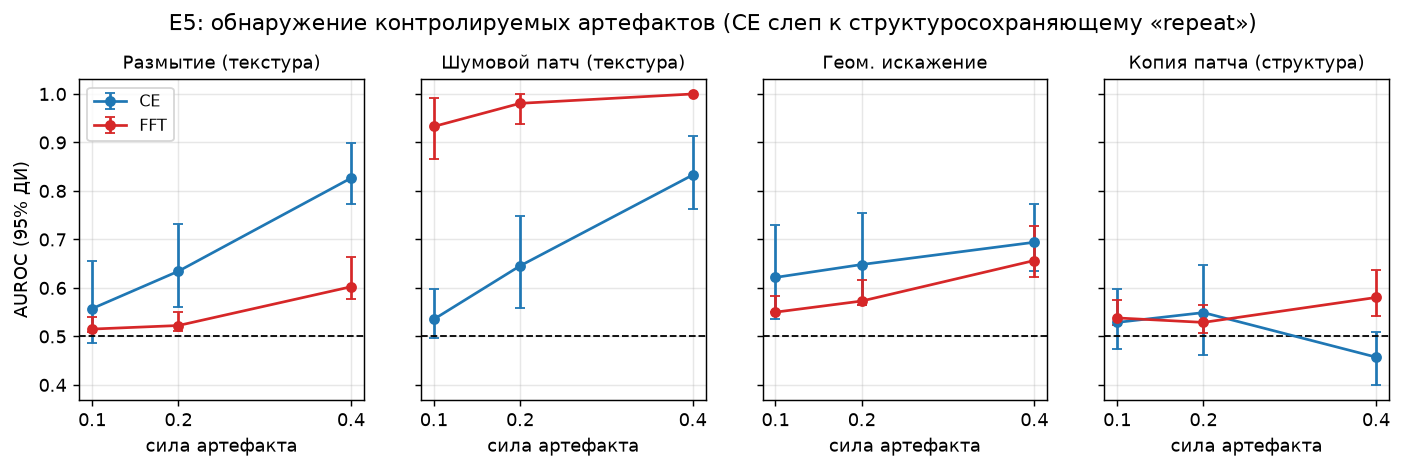
\includegraphics[width=\linewidth]{fig_inject.png}
\caption{Эксперимент 5: AUROC обнаружения контролируемых артефактов как функция силы дефекта
($95\%$ ДИ), CE против радиального спектра Фурье. CE растёт с силой текстурных
дефектов (размытие, шум) и остаётся на уровне случайности для
структуросохраняющей копии патча (правая панель) — аналога семантической
галлюцинации.}
\label{fig:inject}
\end{figure}

\subsection{Эксперимент 6. Эмпирическая проверка предлагаемых расширений}\label{sec:novel_eval}
Четыре расширения из раздела~\ref{sec:extensions} реализованы и проверены тем же
протоколом; для структуросохраняющего случая использован контролируемый артефакт
\texttt{repeat} из эксперимент 5 (группировка кросс-валидации по базовому изображению).
Результаты в таблице~\ref{tab:novel}.

\begin{table}[h!]
\centering
\begin{tabular}{@{}lcccc@{}}
\toprule
Расширение & dim & H1 [95\% ДИ] & H2 [95\% ДИ] & эксперимент 5-\texttt{repeat} [95\% ДИ] \\
\midrule
Б1 сеть переходов        & 4  & 0.790 [0.698, 0.873] & 0.493 [0.355, 0.631] & 0.519 [0.485, 0.564] \\
\textbf{Б2 автокорреляция} & 4  & 0.739 [0.636, 0.829] & 0.606 [0.458, 0.743] & \textbf{0.633 [0.556, 0.720]} \\
Б3 геометрия кривой      & 6  & 0.839 [0.757, 0.911] & 0.440 [0.304, 0.582] & --- \\
Б4 анизотропия           & 60 & 0.804 [0.713, 0.882] & 0.676 [0.546, 0.796]$^{\dagger}$ & --- \\
\bottomrule
\end{tabular}
\caption{Эмпирическая проверка расширений. \textbf{Б2} значимо реагирует на
структуросохраняющее дублирование (нижняя граница ДИ $0{,}556>0{,}5$), которое
гистограмма CE (раздел~\ref{sec:inject}, $0{,}46$) и сеть переходов Б1 ($0{,}52$)
не улавливают. Б3 даёт качество H1 уровня полного $20$-мерного CE на $6$
признаках. Значимость Б4 на H2 ($^{\dagger}$) воспроизводит конфаунд источника
($60$ признаков, $n=67$).}
\label{tab:novel}
\end{table}

Два вывода имеют научную ценность по отдельности. Во-первых, \textbf{Б1
подтверждает} понимание ограничения: матрица переходов остаётся гистограммой пар
шаблонов и инвариантна к сдвигу, поэтому к дублированию слепа так же, как обычная
гистограмма. Во-вторых, \textbf{Б2 опровергает} неизбежность этой слепоты:
нелокальная ординальная автокорреляция значимо реагирует на дублирование,
сохраняя детерминизм и лёгкость. Структуросохраняющие искажения становятся
доступны оценке через нелокальные ординальные дескрипторы.

\paragraph{Развитие Б2.} Базовый дескриптор Б2 дополнен офсетной автокорреляцией
карты ординальных шаблонов: для набора смещений измеряется доля совпадающих
индексов шаблонов сверх случайной коллизии, что задаёт детерминированный сигнал
копирования. Зависимость качества от силы дублирования приведена на
рис.~\ref{fig:b2}. Объединённый дескриптор (блочный и офсетный) даёт лучший
результат — $\mathrm{AUROC}=0{,}660$ при $40\%$ площади — и монотонно растёт с
размером дубля. Тест ДеЛонга \citep{delong1988comparing,sun2014fast} подтверждает
превышение случайности (односторонний $p=0{,}028$); при этом прямое сравнение Б2 с
сетью переходов Б1 пока не достигает значимости ($p=0{,}21$) на $33$ базовых
изображениях, что указывает на потребность в большей выборке.

\begin{figure}[h!]
\centering
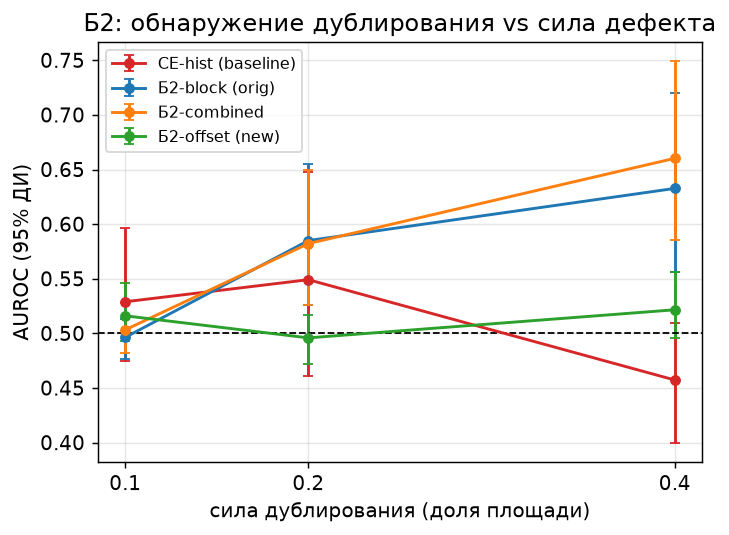
\includegraphics[width=.62\linewidth]{fig_b2.png}
\caption{Развитие Б2: AUROC обнаружения дублирования как функция силы дефекта.
Блочный и объединённый дескрипторы растут с размером дубля; офсетный сам по себе
слаб (текстурная автокорреляция фона), а гистограмма CE остаётся у случайности.}
\label{fig:b2}
\end{figure}

\subsection{Статистическая значимость и множественные сравнения}\label{sec:stats}
Выводы подкреплены тестом ДеЛонга для AUROC и контролем доли ложных открытий. Для
H1 различия CE и базовых методов \emph{не значимы}: CE против спектра Фурье
$p=0{,}82$, против LBP $p=0{,}48$, против объединённого набора $p=0{,}46$ — что
формально подтверждает отсутствие у CE преимущества. Для H2 ни одна из $44$
конфигураций перебора не превышает случайность даже без поправки
(односторонний DeLong-$p<0{,}05$ у $0/44$); после поправки Бенджамини–Хохберга
\citep{benjamini1995controlling} на уровне FDR $0{,}05$ значимых также $0/44$. Это
переводит отказ от H2 из языка доверительных интервалов в формальный тест с
контролем множественных сравнений.

\subsection{Амплитудно-зависимое и мультимасштабное расширения}\label{sec:amethods}
Реализованы два расширения из группы~А (раздел~\ref{sec:extensions}). А1 —
дисперсионная сложность–энтропия: амплитуда вводится через квантование сигнала по
нормальной функции распределения \citep{rostaghi2016dispersion}, далее строится
кривая Реньи по дисперсионным шаблонам. А2 — мультимасштабный двумерный CE: набор
пространственных задержек $\tau_x,\tau_y\in\{1,2,4,8,16\}$ по
\citet{zunino2016discriminating}. В пределах одного датасета ни одно расширение не
улучшает H1 относительно базового CE ($\mathrm{AUROC}$: А1 $0{,}744$, А2 $0{,}776$
против CE $0{,}859$ на собранном корпусе); на низкоразрешённом CIFAKE А2 повышает
качество до $0{,}824$, что согласуется с зависимостью масштабных признаков от
разрешения. Главная ценность расширений и базового CE проявляется в переносе на
независимые данные (раздел~\ref{sec:transfer}).

\subsection{Перенос на независимые датасеты}\label{sec:transfer}
Практическая ценность лёгкого дескриптора состоит в переносимости: тяжёлые
обучаемые детекторы синтетических изображений известны тем, что переобучаются под
конкретный генератор и плохо обобщаются \citep{corvi2023detection}. Поскольку
CE-подобные дескрипторы дают вектор признаков фиксированной размерности
\emph{независимо} от разрешения, перенос между датасетами возможен без
переобучения. Мы обучаем классификатор на одном датасете и применяем его к другому
без подстройки (zero-shot): собранный корпус (256\,px) и CIFAKE (32\,px, иной
генератор). Результаты в таблице~\ref{tab:transfer} и на рис.~\ref{fig:transfer}.

\begin{table}[h!]
\centering
\begin{tabular}{@{}lccccc@{}}
\toprule
Метод & dim & в домене local & в домене CIFAKE & L$\to$C & C$\to$L \\
\midrule
\textbf{CE}                    & 20 & 0.859 & 0.758 & 0.500 & \textbf{0.805} \\
А1 дисперсия                   & 11 & 0.744 & 0.751 & 0.503 & 0.565 \\
А2 мультимасштаб               & 10 & 0.776 & 0.824 & 0.421 & 0.307 \\
тяжёлый набор FFT$+$GLCM$+$LBP  & 71 & 0.891 & 0.942 & 0.614 & 0.175 \\
\bottomrule
\end{tabular}
\caption{Перенос между датасетами (AUROC). Тяжёлый высокоразмерный набор
выигрывает в домене, однако переносится хуже всех: при обучении на CIFAKE и
применении к собранному корпусу его качество падает до $0{,}175$ (ниже
случайности). Базовый CE удерживает $0{,}805$ в этом направлении и остаётся самым
переносимым.}
\label{tab:transfer}
\end{table}

\begin{figure}[h!]
\centering
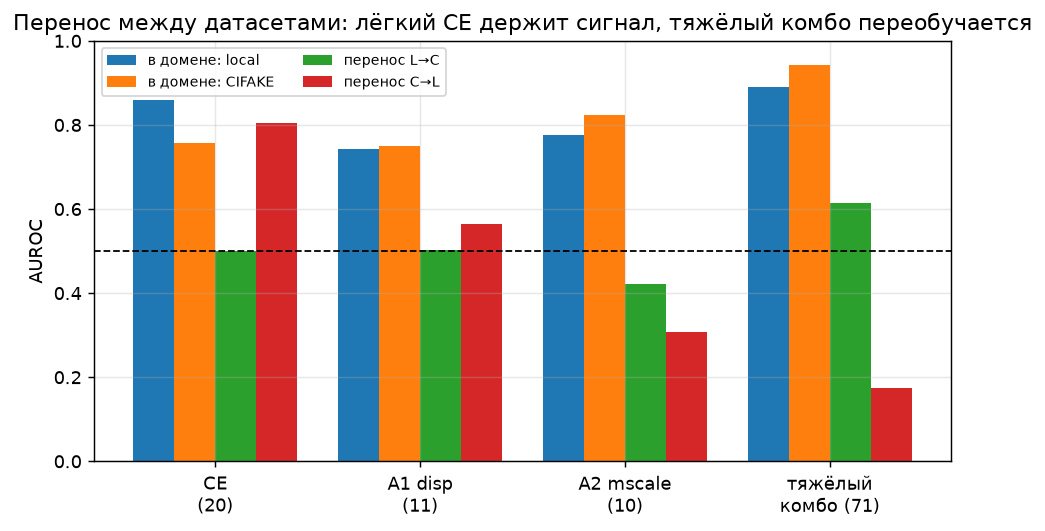
\includegraphics[width=.92\linewidth]{fig_transfer.png}
\caption{Качество в домене и при zero-shot переносе. Тяжёлый набор даёт высшие
столбцы в домене, но его перенос C$\to$L (красный) опускается ниже случайности;
лёгкий CE сохраняет наибольший перенос.}
\label{fig:transfer}
\end{figure}

Картина честная и содержит важные оговорки. Перенос труден для всех методов и
асимметричен: направление L$\to$C близко к случайности, поскольку собранный корпус
мал и многогенераторен, а смена разрешения смещает распределение CE-признаков. При
этом проявляется ясная закономерность: высокоразмерный обучаемый набор переобучается
под датасет и в направлении C$\to$L опускается до $0{,}175$, тогда как лёгкий
$20$-мерный CE сохраняет $0{,}805$ и деградирует наиболее мягко. Это подкрепляет
тезис о переносимости лёгких ординальных дескрипторов: знание о статистике
«реальное против синтетического» переносится у CE лучше, чем у тяжёлого отпечатка.

Контрольный эксперимент уточняет границы этого вывода. При приведении обоих
датасетов к общему разрешению ($32$, $64$, $128$\,px) перенос не восстанавливается
систематически: качество C$\to$L для CE колеблется в пределах $0{,}16$–$0{,}38$ и
зависит от выбранного разрешения, а понижение разрешения собранного корпуса само по
себе ослабляет внутридоменный сигнал. Беспороговый скор Махаланобиса деградирует
мягче обучаемого классификатора, оставаясь умеренным ($0{,}55$–$0{,}63$). Надёжный
кросс-датасетный перенос между столь разными источниками (веб-фотографии против
CIFAR, много генераторов против одного) остаётся открытой задачей; чистая проверка
требует кросс-генераторного переноса при фиксированном разрешении.

\subsection{Оценка искажения относительно реальных изображений}\label{sec:distortion}
Сигнал H1 допускает беспороговую формулировку. По CE-признакам реальных
изображений оценивается гауссовское многообразие (среднее и ковариация с
регуляризацией Ледуа–Вольфа), а \emph{квадрат расстояния Махаланобиса} до него
служит непрерывной мерой искажения. Эта мера разделяет реальные и синтетические
изображения почти как обучаемый классификатор: $\mathrm{AUROC}=0{,}815$, при медиане
расстояния $1{,}3$ для реальных против $12{,}6$ и $12{,}8$ для удачных и неудачных
генераций (синтетика примерно в десять раз дальше от многообразия). При
управляемом внесении искажений в реальные изображения мера растёт монотонно
(размытие: $1\to563\to11846$; шум: $1\to14{,}6\to30$), что подтверждает её
интерпретацию как меры искажения.

Дополнительный тест проясняет природу синтетического следа. Вдоль оси
линейного дискриминанта (реальные против синтетических) размытые реальные
изображения ($\sigma=2$) смещаются на сторону синтетических (все $100\%$
пересекают медиану реальных), тогда как зашумлённые остаются на стороне реальных.
Низкочастотное искажение приближает реальное изображение к синтетическому, что
согласуется с известным фактом о пониженных высоких частотах диффузионных
генераций \citep{corvi2023detection,tan2025fractal}.

% ==================================================================
\subsection*{Выводы по главе}
Гипотеза H1 подтверждается внутри доменов, но контроль источника выявляет
конфаунд, а CE не превосходит спектр Фурье. Гипотеза H2 отвергается на всех 44
конфигурациях; контролируемая инъекция артефактов вскрывает механизм — слепоту
глобальной статистики к структуросохраняющему дублированию. Кросс-датасетный
перенос остаётся ограниченным.

\section{Прикладной метод: ординальный детектор дублирования}\label{sec:copymove}

Единственный положительный сигнал по структурным дефектам (Б2) мы доводим до
самостоятельного \emph{лёгкого детерминированного} метода локализации копирования
(copy-move). Метод полностью укладывается в ограничения $<1$ ГБ ОЗУ и работает
$\approx0{,}45$ с на изображение $256\times256$.

\paragraph{Алгоритм.} По изображению строится карта двумерных ординальных шаблонов
$P$ (индексы $2\times2$-окон). Каждый блок $10\times10$ карты $P$ с достаточным
разнообразием шаблонов хэшируется; одинаковые блоки, удалённые друг от друга,
голосуют за вектор смещения между ними. Пик голосования даёт \emph{точное}
смещение копии $\delta^{*}$; маска дубля строится из точных совпадений
$P(p)=P(p+\delta^{*})$ морфологической чисткой и отбором связных компонент. Всё
детерминировано и линейно по числу пикселей.

\paragraph{Ключевое свойство.} По лемме~\ref{lem:mono} ординальные шаблоны
инвариантны к монотонной тоновой правке. Поэтому метод устойчив к типичному приёму
маскировки подделки — изменению яркости или гаммы вставленного фрагмента, — на
котором ломаются методы, основанные на интенсивностях. Мы сравниваем ординальный
детектор с тем же конвейером, применённым к квантованным \emph{интенсивностям}.

\begin{table}[h!]
\centering
\begin{tabular}{@{}lcccc@{}}
\toprule
& \multicolumn{2}{c}{ординальный} & \multicolumn{2}{c}{интенсивностный} \\
\cmidrule(lr){2-3}\cmidrule(lr){4-5}
Условие & лок.\ F1 & детекция AUROC & лок.\ F1 & детекция AUROC \\
\midrule
точная копия       & 0.906 & 0.966 & 0.843 & 0.855 \\
копия + гамма $2{,}2$  & \textbf{0.870} & \textbf{0.950} & 0.020 & 0.499 \\
копия + гамма $0{,}45$ & \textbf{0.863} & \textbf{0.965} & 0.017 & 0.500 \\
\bottomrule
\end{tabular}
\caption{Локализация и детекция copy-move ($33$ изображения, площадь дубля $8\%$).
Без тоновой правки оба метода работают; при монотонной правке вставки
интенсивностный детектор падает до случайности, а ординальный сохраняет
$\mathrm{F1}\approx0{,}87$ и $\mathrm{AUROC}\approx0{,}95$.}
\label{tab:copymove}
\end{table}

\begin{figure}[h!]
\centering
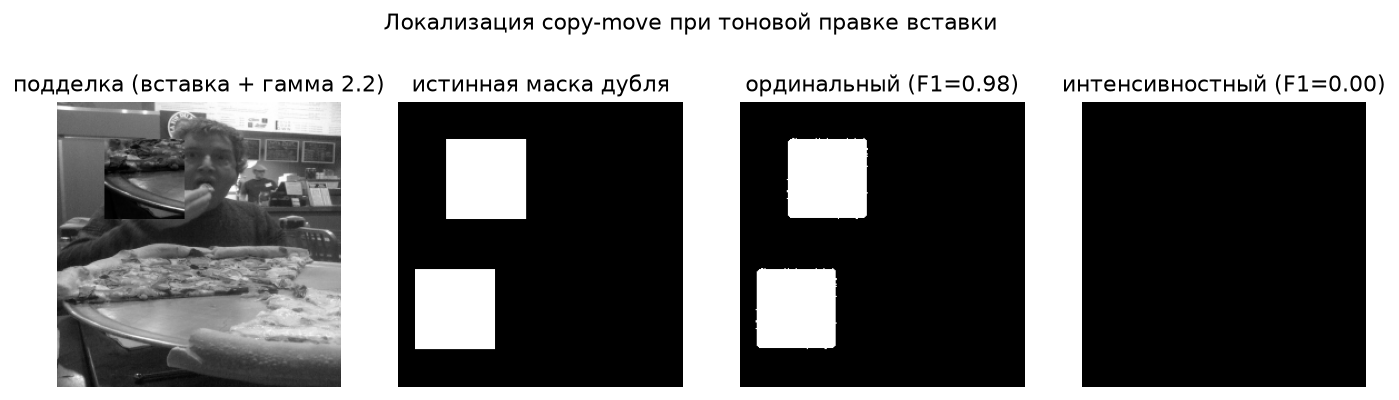
\includegraphics[width=\linewidth]{fig_copymove_qual.png}
\caption{Локализация при тоновой правке вставки (гамма $2{,}2$). Ординальный
детектор находит исходную и вставленную области; интенсивностный — нет.}
\label{fig:copymove}
\end{figure}

\paragraph{Применимость и границы.} Метод полезен как лёгкий
детерминированный инструмент контроля качества и форензики: он локализует
дублированные области и устойчив к тоновой маскировке, не требует обучения и
переносится между изображениями без подстройки. Ограничения честны: он рассчитан
на \emph{близкие к точным} копии. Частичное снятие этого ограничения дано ниже.

\subsection{Инвариантность к геометрии вставки}\label{sec:copymove_inv}
Точное хэширование осевых блоков не выдерживает геометрических преобразований
вставки. Мы добавляем инвариантный вариант: вокруг каждого пикселя берутся $N=8$
точек на концентрических кольцах, вычисляются их ранги, и дескриптором служит
\emph{канонический минимум} по диэдральной группе (циклические сдвиги и
отражение) последовательности рангов. Поворот изображения сдвигает кольцо
циклически, отражение обращает его порядок, поэтому канонизация даёт
инвариантность к отражению и повороту, а ранги сохраняют монотонную инвариантность
(лемма~\ref{lem:mono}); несколько радиусов дают терпимость к масштабу. Пиксели,
чей дескриптор повторяется на удалении и образует связную область, помечаются как
дубль.

\begin{table}[h!]
\centering
\begin{tabular}{@{}lcccc@{}}
\toprule
& \multicolumn{2}{c}{кольцевой (инвариантный)} & \multicolumn{2}{c}{блочный (только сдвиг)} \\
\cmidrule(lr){2-3}\cmidrule(lr){4-5}
Геометрия вставки & лок.\ F1 & детекция & лок.\ F1 & детекция \\
\midrule
сдвиг            & 0.381 & 0.856 & \textbf{0.857} & \textbf{0.950} \\
отражение        & \textbf{0.375} & \textbf{0.856} & 0.015 & 0.516 \\
поворот $90^\circ$ & \textbf{0.380} & \textbf{0.858} & 0.000 & 0.500 \\
поворот $30^\circ$ & 0.024 & 0.459 & 0.000 & 0.500 \\
масштаб $0{,}8$    & 0.029 & 0.499 & 0.000 & 0.500 \\
\bottomrule
\end{tabular}
\caption{Детекция/локализация copy-move при геометрической правке вставки
(детекция — AUROC). Кольцевой дескриптор добавляет инвариантность к отражению и
повороту на $90^\circ$ (детекция $\approx0{,}86$, где блочный метод у случайности)
ценой более грубой локализации. Произвольный поворот и масштаб остаются
недостижимыми для точного ординального сопоставления.}
\label{tab:copymove_inv}
\end{table}

\begin{figure}[h!]
\centering
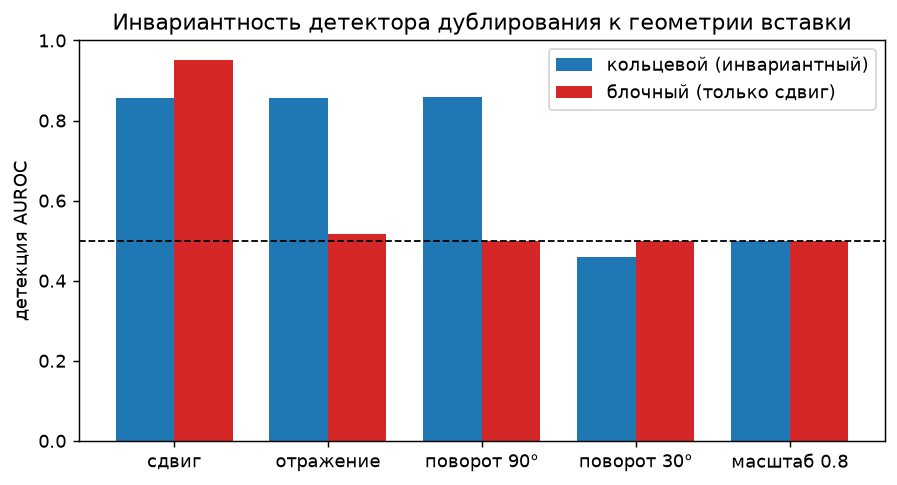
\includegraphics[width=.78\linewidth]{fig_copymove_inv.png}
\caption{Детекция дублирования при разной геометрии вставки. Кольцевой
дескриптор устойчив к отражению и повороту $90^\circ$; оба метода теряют сигнал на
произвольном повороте и масштабе.}
\label{fig:copymove_inv}
\end{figure}

Методы комплементарны: блочный даёт точную локализацию для сдвига и тоновой правки,
кольцевой добавляет диэдральную инвариантность при более грубой локализации.
Инвариантность к произвольному повороту и масштабу требует нечёткого (приближённого)
сопоставления дескрипторов и оставлена развитию.

\subsection{Калибровка порога решающего правила}\label{sec:copymove_thr}
Решающее правило детектора использует один порог по скору (доле площади
совпадений). Чтобы избежать смещения отбора, базовые изображения разбиты на
обучающую и отложенную части ($60/40$) \emph{без утечки}: каждое базовое
изображение целиком попадает в одну часть. Порог подбирается на обучающей части
(по максимуму $F_1$ и по критерию Юдена), метрики рабочей точки приводятся на
отложенной (таблица~\ref{tab:thr}). Беспороговый AUROC на отложенной части
составляет $0{,}959$.

\begin{table}[h!]
\centering
\begin{tabular}{@{}lccccc@{}}
\toprule
Порог (обучение) & точность & полнота & $F_1$ & сбал.\ точность & MCC \\
\midrule
макс.\ $F_1$ ($t=0{,}068$)   & 0.929 & 0.929 & 0.929 & 0.929 & 0.857 \\
критерий Юдена ($t=0{,}097$) & 1.000 & 0.857 & 0.923 & 0.929 & 0.866 \\
\bottomrule
\end{tabular}
\caption{Метрики рабочей точки на отложенной части (порог подобран на обучающей,
разбиение по базовым изображениям). Калиброванный порог $\approx0{,}07$--$0{,}10$
доли площади совпадений даёт $F_1\approx0{,}93$ и MCC$\,\approx0{,}86$; критерий
Юдена даёт нулевую долю ложных срабатываний при чуть меньшей полноте.}
\label{tab:thr}
\end{table}

% ==================================================================
\subsection*{Выводы по главе}
На основе нелокальных ординальных признаков построен лёгкий детерминированный
детектор-локализатор дублирования. Он устойчив к тоновой правке вставки (следствие
монотонной инвариантности) и в кольцевом варианте — к отражению и повороту на
90 градусов; произвольный поворот и масштаб остаются ограничением.

\section{Обсуждение}\label{sec:discussion}

Результаты переворачивают исходную интерпретацию. То, что ранее подавалось как
«детектор галлюцинаций» с «побочным эффектом» различения синтетики, на деле
сводится к \emph{оценке синтетичности}, а заявленной способности обнаруживать
галлюцинации в данных \emph{нет}. Это согласуется с физикой явления: реальные и
синтетические изображения различаются устойчивыми частотно-текстурными
характеристиками \citep{corvi2023detection}, которые порядковые шаблоны улавливают;
семантические же галлюцинации (лишний палец, нечитаемый текст) не меняют
глобальную порядковую статистику и потому невидимы для CE. эксперимент 5
(раздел~\ref{sec:inject}) делает этот механизм наглядным: CE «видит» дефекты,
искажающие локальную текстуру, но слеп к структуросохраняющему дублированию —
именно к тому классу искажений, к которому относятся семантические галлюцинации.

Не менее важно, что сравнение с базовыми методами (эксперимент 4) показывает: на задаче H1
CE \emph{не превосходит} тривиальный спектр Фурье. Следовательно, ценность CE
состоит в дешевизне и интерпретируемости при сопоставимом качестве; претензия на
уникальную диагностическую способность не подтверждается. Маргинальная значимость
высокоразмерного объединённого набора на H2 объясняется конфаундом источника
между классами; контролируемый эксперимент это подтверждает.

Параметрический анализ отвечает на вопрос, вынесенный в заголовок: качество
CE-оценки определяется прежде всего \emph{задержкой} ($\tau=1$) и \emph{схемой
линеаризации} (горизонтальный растр), тогда как размерность вложения и переход к
нативным 2D-шаблонам второстепенны. Эти зависимости воспроизводимы между двумя
независимыми датасетами.

Наконец, выявленный дефект исходного конвейера (необучаемая случайная свёртка,
раздел~\ref{sec:fix}) — методологический урок: дешёвую эвристику легко принять за
работающий метод, если оценивать её неподходящей метрикой на малой выборке. Строгий
протокол с доверительными интервалами устраняет этот риск.

% ==================================================================
\section{Математические расширения метода и новые идеи}\label{sec:extensions}

Все предложения ниже сохраняют ключевые свойства метода — \emph{лёгкость,
скорость, детерминизм}: они развивают \emph{математику} дескриптора и не вводят
обучаемых параметров. Предложения разделены на (А) улучшения, опирающиеся на
литературу, и (Б) оригинальные идеи, не встречавшиеся в данном контексте.
Оригинальные расширения реализованы и проверены эмпирически
(раздел~\ref{sec:novel_eval}, таблица~\ref{tab:novel}); ключевые наблюдения
отмечены ниже по месту.

\subsection{Улучшения на основе литературы}

\paragraph{А1. Амплитудно-зависимые ординальные признаки.}
Классические шаблоны Бандта–Помпе отбрасывают амплитуду. Замена их взвешенной
\citep{fadlallah2013weighted}, амплитудно-зависимой \citep{azami2016amplitude} или
дисперсионной \citep{rostaghi2016dispersion} энтропией возвращает информацию о
контрасте. \emph{Гипотеза:} пересглаживание (low-pass) диффузионных изображений
оставляет амплитудный след, который усилит H1; контраст­ные аномалии локальных
галлюцинаций потенциально дают сигнал и для H2. Стоимость — та же $O(N)$.

\paragraph{А2. Мультимасштабный 2D-CE.}
Вслед за \citet{zunino2016discriminating} ввести пространственные задержки
$\tau_x,\tau_y\in\{1,2,4,8,\dots\}$ и конкатенировать CE-кривые по масштабам.
Артефакты повышающей дискретизации локализованы по частоте/масштабу, поэтому
мультимасштабный признак должен повышать и устойчивость H1, и кросс-генераторную
обобщаемость, перекликаясь с самоподобием спектра \citep{tan2025fractal}.

\paragraph{А3. Локальные CE-карты с пулингом.}
Вместо одного глобального вектора вычислять CE по скользящим патчам, получая
\emph{карту} $(H,C)$, и агрегировать её порядковыми статистиками (среднее,
максимум, перцентили). Это детерминированный аналог идеи мультигранулярных
энтропийных карт MLEP \citep{yuan2025mlep} без обучаемой CNN. Максимум-пулинг
локальной сложности — прямой рычаг против \emph{локальных} галлюцинаций, которые
глобальная статистика усредняет (ограничение, выявленное в эксперимент 5).

\subsection{Оригинальные идеи}

\paragraph{Б1. Ординальные сети переходов для изображений (главная идея).}
Гистограмма ординальных шаблонов \emph{инвариантна к перестановке и сдвигу} — и
именно поэтому слепа к дублированию (механизм провала H2 и артефакта
\texttt{repeat} в эксперимент 5). Предлагается перейти от гистограммы к \emph{графу переходов}
между соседними двумерными шаблонами и извлекать его инварианты (энтропия
распределения рёбер, дисбаланс степеней, доля повторяющихся мотивов). Копия патча
порождает аномальные повторяющиеся переходы, невидимые для гистограммы. Это
\emph{принципиальная} атака на структурную слепоту CE, оставающаяся
детерминированной и линейной (подсчёт переходов). Эмпирически (эксперимент 6) этот вариант
подтвердил ограничение: матрица переходов сама остаётся гистограммой, поэтому к
дублированию слепа.

\paragraph{Б2. Нелокальная ординальная автокорреляция (детектор дублирования).}
Детерминированный дескриптор, измеряющий повторяемость блоков ординальных шаблонов
по изображению (ординальный block-matching). Он прямо нацелен на
структуросохраняющие артефакты дублирования (случай \texttt{repeat}), которые
локальная CE-гистограмма принципиально не видит, — детектор повтора без обучения.
Эмпирически (эксперимент 6) этот вариант значимо реагирует на дублирование
($\mathrm{AUROC}=0{,}633$, нижняя граница ДИ выше $0{,}5$), снимая ограничение,
подтверждённое для Б1.

\paragraph{Б3. Геометрия кривой Реньи как признак.}
Кривые Реньи стохастических процессов имеют положительную кривизну у начала, а
хаотических — отрицательную \citep{RePEc:eee:phsmap:v:498:y:2018:i:c:p:74-85}.
Вместо подачи «сырых» $(H_\alpha,C_\alpha)$ извлекать \emph{геометрические
инварианты} кривой (начальный наклон, кривизну, длину дуги) — компактные,
интерпретируемые, детерминированные признаки меньшей размерности.

\paragraph{Б4. CE-анизотропия.}
Поскольку артефакты дискретизации выровнены по осям, разность CE, посчитанных вдоль
горизонтального, вертикального и диагонального обходов, сама по себе является
признаком синтетичности. Наш перебор уже намекает на это (\texttt{row}$\neq$%
\texttt{diag}); формализация \emph{зазора} как одномерного дешёвого признака
прямо мотивирована частотным механизмом из раздела~\ref{sec:related}.

\subsection{Пересмотр метрик}\label{sec:metrics}
Исходная эвристика $\text{score}(\Theta)$ заменена на AUROC/AP. Для полноты
предлагается добавить: (i) пороговые метрики классификации — сбалансированную
точность, $F_1$ и коэффициент Мэтьюса (MCC), устойчивый при дисбалансе; (ii)
\emph{калибровку} — ожидаемую калибровочную ошибку (ECE) и оценку Бриера, важные
для риск-ориентированного использования; (iii) \emph{меры близости} как
безпороговый, неконтролируемый скоринг: расстояние Махаланобиса от точки до
распределения CE-признаков реальных изображений, энергетическое расстояние или
MMD между распределениями признаков классов. Последнее возвращает исходную идею
«огибающей» реальных данных, но придаёт ей строгую вероятностную форму и
сохраняет детерминизм.

% ==================================================================
\section{Ограничения и направления будущей работы}\label{sec:future}
\begin{itemize}
\item \textbf{Сильные представления.} Сравнение с дешёвыми признаками выполнено
      (раздел~\ref{sec:baselines}); следующий шаг — сопоставление с сильными
      обучаемыми представлениями (CLIP/DINOv2 + логистическая регрессия), чтобы
      оценить верхнюю границу качества различения синтетических изображений на тех же данных.
\item \textbf{Кросс-генераторная обобщаемость.} Проверка на GenImage (множество
      генераторов) покажет, переносится ли сигнал между семействами моделей.
\item \textbf{Свободный от конфаунда корпус.} Контроль источника
      (раздел~\ref{sec:confound}) показал, что метаданные файла разделяют классы
      собранного корпуса; нужен сбор с единым пайплайном (одинаковые формат,
      разрешение, сжатие) и публикуемым datasheet, чтобы H1 измерял синтетичность,
      а не происхождение.
\item \textbf{Данные с семантическими галлюцинациями.} эксперимент 5 моделирует
      \emph{структурные} дефекты; нужен корпус с размеченными \emph{семантическими}
      галлюцинациями (парные генерации одного генератора с известной ошибкой счёта
      объектов или несоответствием промпту), чтобы проверить H2 на целевом явлении.
\item \textbf{Выбор параметров без смещения отбора.} Лучшая из $44$ конфигураций
      выбрана на тех же данных, что создаёт риск selection bias; для итоговых чисел
      желателен вложенный (nested) CV либо заранее зафиксированный критерий выбора и
      отдельный тестовый набор.
\item \textbf{Сильные представления как верхняя граница.} Сравнение с
      CLIP/DINOv2 и простыми CNN/ViT-признаками по тому же протоколу покажет цену
      интерпретируемости CE.
\item \textbf{Устойчивость к постобработке.} Стресс-тест к JPEG/WebP-сжатию,
      передискретизации, кадрированию и удалению метаданных — для forensic-задач это
      часть предмета.
\item \textbf{Калибровка и риск-метрики.} Для QA-применения нужны Brier, ECE, MCC и
      сбалансированная точность с анализом порогов.
\end{itemize}

% ==================================================================
\subsection*{Выводы по главе}
Обсуждение связывает эмпирику с доказанными свойствами: CE измеряет статистику
синтетичности и слеп к семантике; практическую ценность несут нелокальные
ординальные признаки. Намечены направления развития и очерчены ограничения данных
и протокола.

\section{Заключение}\label{sec:conclusions}

В работе систематически изучено влияние параметров методов на основе
сложности–энтропии на оценку ошибок генерации диффузионных моделей. Вместо
эвристической метрики применён более строгий и воспроизводимый протокол
(логистическая регрессия, повторная стратифицированная кросс-валидация,
бутстреп-доверительные интервалы, тест ДеЛонга и контроль доли ложных открытий), а
задача поставлена как раздельная проверка двух гипотез по явной таксономии ошибок.
Основной вывод: \textbf{CE-кривые служат дешёвым и интерпретируемым дескриптором
синтетичности}, который различает реальные и синтетические изображения внутри
домена (AUROC до $0{,}858$ на собранном корпусе и $0{,}756$ на сбалансированном
CIFAKE) и управляется прежде всего задержкой $\tau$ и схемой линеаризации, однако
не превосходит тривиальный спектр Фурье. Контроль источника показал, что
внутридоменные числа H1 частично завышены конфаундом данных, поэтому надёжной
оценкой служит сбалансированный CIFAKE. \textbf{Глобальная CE-статистика не решает
задачу обнаружения семантических галлюцинаций}: ни одна из $44$ конфигураций не
превышает случайность значимо (DeLong, FDR), а контролируемая инъекция артефактов
показывает чувствительность к текстурным дефектам при слепоте к
структуросохраняющему дублированию. Для структурных дефектов перспективны
нелокальные ординальные признаки: на их основе построен \textbf{прикладной
детерминированный детектор-локализатор дублирования} (copy-move), который
локализует копии с $\mathrm{F1}\approx0{,}9$ и, благодаря монотонной инвариантности
(лемма~\ref{lem:mono}), устойчив к тоновой маскировке вставки, где интенсивностные
методы падают до случайности. Дополнительно выявлен и устранён методологический
дефект исходного конвейера. Полученные результаты дают воспроизводимую основу для
кросс-генераторной проверки и сбора свободного от конфаунда размеченного корпуса.

\clearpage
\addcontentsline{toc}{section}{Список литературы}
\bibliography{references}

\clearpage
\appendix
\section{Полная таблица параметрического перебора}
\label{app:sweep}
Полные результаты ($44$ параметризации $\times$ две задачи) с доверительными
интервалами приведены в сопровождающем файле \texttt{paper/results/sweep.csv}.
Ниже — сводка по схемам линеаризации для задачи H1 при $\tau=1$.

\begin{table}[h!]
\centering
\begin{tabular}{@{}lccc@{}}
\toprule
Схема & среднее AUROC & min & max \\
\midrule
\texttt{snake}   & 0.844 & 0.837 & 0.855 \\
\texttt{row}     & 0.842 & 0.832 & 0.858 \\
\texttt{col}     & 0.799 & 0.780 & 0.816 \\
\texttt{hilbert} & 0.798 & 0.768 & 0.823 \\
\texttt{diag}    & 0.770 & 0.754 & 0.784 \\
\bottomrule
\end{tabular}
\caption{Влияние схемы линеаризации на задачу H1 (real vs synthetic) при
$\tau=1$, агрегировано по $d\in\{3,4,5,6\}$.}
\label{tab:scheme}
\end{table}

\end{document}
